% This is LLNCS.DEM the demonstration file of
% the LaTeX macro package from Springer-Verlag
% for Lecture Notes in Computer Science,
% version 2.4 for LaTeX2e as of 16. April 2010
%
\documentclass[runningheads]{llncs}
%

%% Save the class definition of \subparagraph
\let\llncssubparagraph\subparagraph
%% Provide a definition to \subparagraph to keep titlesec happy
\let\subparagraph\paragraph
%% Load titlesec
\usepackage[compact]{titlesec}
%% Revert \subparagraph to the llncs definition
\let\subparagraph\llncssubparagraph
\usepackage{makeidx}  % allows for indexgeneration
\usepackage{url}
\usepackage[xetex]{hyperref}
\usepackage{todonotes}
\usepackage{listings}
% \usepackage{fontspec}
\usepackage{fancyvrb}
\usepackage[labelfont=bf]{caption}
\usepackage{subcaption}
\captionsetup{compatibility=false}
\usepackage{times}
\usepackage[scaled=0.875]{inconsolata}
\usepackage{graphicx}
\usepackage{xcolor}
\usepackage{lipsum}
\usepackage{booktabs}

\newcommand{\comment}[1]{}

% Member sequences
\newcommand{\seq}[1]{\overline{#1}}

% arrays
\newcommand{\ba}{\begin{array}}
\newcommand{\ea}{\end{array}}
\newcommand{\bda}{\[\ba}
\newcommand{\eda}{\ea\]}
\newcommand{\ei}{\end{array}}
\newcommand{\bcases}{\left\{\begin{array}{ll}}
\newcommand{\ecases}{\end{array}\right.}
\newcommand{\sporeurl}{\url{https://github.com/scala/spores}}
% spacing
\newcommand{\gap}{\quad\quad}
\newcommand{\andalso}{\quad\quad}
\newcommand{\biggap}{\quad\quad\quad}
\newcommand{\nextline}{\\ \\}
\newcommand{\htabwidth}{0.5cm}
\newcommand{\tabwidth}{1cm}
\newcommand{\htab}{\hspace{\htabwidth}}
\newcommand{\tab}{\hspace{\tabwidth}}
\newcommand{\linesep}{\ \hrulefill \ \smallskip}

\newcommand{\ie}{{\em i.e.,~}}
\newcommand{\eg}{{\em e.g.,~}}
\newcommand{\etc}{{\em etc}}

\newcommand*\loc{
\includegraphics[height=0.65em,keepaspectratio]{loc}}
\newcommand*\stars{
\includegraphics[height=0.8em,keepaspectratio]{stars}}
\newcommand*\contribs{
\includegraphics[height=0.8em,keepaspectratio]{contribs}}

\lstdefinelanguage{Scala}%
{morekeywords={abstract,case,catch,char,class,%
    def,else,extends,final,%
    if,import,%
    match,module,new,null,object,override,package,private,protected,%
    public,return,super,this,throw,trait,try,type,val,var,with,implicit,%
    macro,sealed,%
  },%
  sensitive,%
  morecomment=[l]//,%
  morecomment=[s]{/*}{*/},%
  morestring=[b]",%
  morestring=[b]',%
  showstringspaces=false%
}[keywords,comments,strings]%

% \lstset{language=Scala,%
%   mathescape=true,%
%   columns=[c]fixed,%
%   numbers=left, numberstyle=\scriptsize\color{gray}\ttfamily,
%   basewidth={0.5em, 0.40em},%
%   basicstyle=\tt,%
%   xleftmargin=0.0cm
% }

% \setmainfont[
%   Ligatures=TeX,
%   SmallCapsFont={TeX Gyre Termes},
%   SmallCapsFeatures={Letters=SmallCaps},
% ]{Times New Roman}

\lstset{tabsize=2,
basicstyle=\ttfamily\fontsize{9pt}{1em}\selectfont,
commentstyle=\itshape\rmfamily,
numbers=left, numberstyle=\scriptsize\color{gray}\ttfamily, language=scala,moredelim=[il][\sffamily]{?},mathescape=false,showspaces=false,showstringspaces=false,xleftmargin=15pt,escapechar=@, morekeywords=[1]{let,fn,val},deletekeywords={for},classoffset=0,belowskip=\smallskipamount
}

\definecolor{light-gray}{gray}{0.80}
\definecolor{lightGray}{rgb}{0.9, 0.9, 0.9}

\newcommand{\Hilight}{\makebox[0pt][l]{\color{light-gray}\rule[-0.45em]{\linewidth}{1.5em}}}

% \setlength{\belowcaptionskip}{-5pt}
\setlength{\textwidth}{12.4cm}
 \setlength\intextsep{ 0pt plus 2pt minus 2pt}

% \titlespacing{\section}{0pt}{\parskip}{-\parskip}

\begin{document}

% \fontspec[
%   SmallCapsFont={TeX Gyre Termes},
%   SmallCapsFeatures={Letters=SmallCaps},
% ]{Times New Roman}
\VerbatimFootnotes
% \setmonofont[Scale=0.8,BoldFont={Consolas Bold}]{Consolas}

%
\mainmatter              % start of the contributions


\title{Reactive Join Patterns}

\titlerunning{Reactive Join Patterns}  % abbreviated title (for running head)
%                                     also used for the TOC unless
%                                     \toctitle is used
%
\author{Philipp Haller$^{1}$ \and Alon Dolev$^{2}$\footnote{Work done while at TU Delft.}
\and Heather Miller$^{3}$}

%%% list of authors for the TOC (use if author list has to be modified)
\tocauthor{Philipp Haller, Alon Dolev, and Heather Miller}

% \institute{EPFL and Typesafe, Inc$^{1}$\\

% \texttt{\scriptsize \{heather.miller, martin.odersky\}@epfl.ch}
% and \texttt{\scriptsize philipp.haller@typesafe.com}$^{1}$}

% Ergon Informatik AG
% Merkurstrasse 43
% 8032 Zürich


\institute{KTH Royal Institute of Technology, Sweden$^{1}$\\
% \texttt{phaller@kth.se}\\
Ergon Informatik AG, Switzerland$^{2}$\\
% \texttt{alon@dolev.ch}\\
EPFL, Switzerland$^{3}$\\
% \texttt{heather.miller@epfl.ch}
}


\setlength{\abovecaptionskip}{0pt}
\setlength{\belowcaptionskip}{0pt}
\authorrunning{P. Haller, A. Dolev, and H. Miller} % abbreviated author list (for running head)

\maketitle              % typeset the title of the contribution

\begin{sloppypar}
\begin{abstract}

Asynchronous programming has been a long-standing challenge. Meanwhile, the
rise of asynchronous, event-based programming, as witnessed, \eg by the
Reactive Manifesto, has propelled stream-based programming into the focus of
mainstream software development.

This paper proposes a new approach to {\em scalable and declarative
synchronization of asynchronous event streams} based on join
patterns. Instead of introducing a new, incompatible
programming model, we present a new synchronization construct for an existing,
widely-used programming model for asynchronous streams. In order to support
the ordering constraints of streams, we adapt Turon and Russo's scalable
join-pattern matching algorithm. Furthermore, our join
synchronization construct enables integrating with flow-control mechanisms of
stream-based programming models. Thus, our implementation of join patterns is the
first to support bounded message buffers. Experimental results using micro
benchmarks show an average increase in throughput of 30-36\% compared to
the standard joins implementation of \textsc{RxJava}, a state-of-the-art
streaming implementation for the JVM.

\keywords{concurrent programming, join-calculus, streams}
\end{abstract}


\section{Introduction}
\label{sec:introduction}

Asynchronous programming has been a long-standing challenge. A multitude of
programming models has been proposed to simplify the task, including
actors~\cite{Hewitt77}, futures~\cite{Halstead85}, promises~\cite{LiskovS88},
and join patterns~\cite{Fournet:1996}. The asynchronous models of
F\#~\cite{SymePL11}, C\#~\cite{FormalizingAsync}, and
Scala~\cite{ScalaAsyncSIP} provide language support for programming with
futures (or ``tasks'') by avoiding an inversion of control that is inherent
in designs based on callbacks~\cite{John88a}.

Meanwhile, the rise of asynchronous, event-based programming as witnessed, \eg
by the Reactive Manifesto~\cite{ReactiveManifesto}, has propelled stream-based
programming into the focus of mainstream software development. As a result,
asynchronous language extensions have been extended to streams, \eg in
Scala~\cite{RAY} and Dart~\cite{MeijerMB15}. However, the scalable
synchronization of streams using fine-grained concurrent algorithms has
remained a challenge.

This paper proposes a new approach to {\em scalable and declarative synchronization
of asynchronous event streams} based on join patterns~\cite{Fournet:1996}. Instead of
introducing a new, incompatible programming model, we present a new
synchronization construct for an existing, widely-used programming model for
asynchronous streams. In order to support the ordering constraints of streams,
we adapt Turon and Russo's scalable join-pattern matching algorithm~\cite{Turon:2011}. Furthermore,
our join synchronization construct enables integrating with flow-control
mechanisms of stream-based programming models, such as \textsc{RxJava}~\cite{RxJava}
and Reactive Streams~\cite{ReactiveStreams}. Experimental results using micro
benchmarks show an average increase in throughput of 30-36\% compared to
\textsc{RxJavaJoins}~\cite{RxJavaJoins}, the standard, industrial-strength joins
implementation of \textsc{RxJava}.


\subsection{Related work}\label{sec:related}

\begin{table}[h]
\centering
\resizebox{\textwidth}{!}{%
\begin{tabular}{@{}llllllll@{}}
\toprule
 & Language & Implementation & Synchrony & Choice & Channels & Concurrency & Buffers \\ \midrule
Polyphonic C\#         & C\# & Compiler & Both & Non-Determ. & Methods & Coarse & Unbounded \\
JoinJava               & Java & Compiler & Both & Both & Methods & Coarse & Unbounded \\
C\# Joins Library      & .NET & Library & Both & Non-Determ. & Channels & Coarse & Unbounded \\
Scala Joins            & Scala & Library & Both & Non-Determ. & Channels & Coarse & Unbounded \\
JErlang                & Erlang & Both & Async & Deterministic & Messages & Coarse & Unbounded \\
Scalable Join Patterns & C\# & Library & Both & Non-Determ. & Channels & Fine & Unbounded \\
RxJavaJoins            & Java & Library & Async & Non-Determ. & Observables & Coarse & Unbounded \\
This paper             & Scala & Macro & Async & Both & Observables & Fine / Coarse & Both \\ \bottomrule
\end{tabular}
}
\caption{Related join-calculus implementations}
\label{tab:JoinCalculusImplementations}
\end{table}

Table~\ref{tab:JoinCalculusImplementations} gives an overview of join-calculus
implementations most closely related to our work.
In general, we differ from stand-alone and extended compiler implementations
by leveraging static meta-programming. With the use of Scala macros~\cite{burmako13}
our \verb|join| synchronization construct
can be imported like a regular library. This means that users do not have to
install and possibly maintain compiler extensions (or a whole new compiler)
for projects where only parts require the provided functionality. Further, the
macros we use do not allow changing the syntax of the host language (in this case, Scala);
this means, clients of our system use a syntax that is already familiar, helping adoption.
In contrast, both JoinJava~\cite{Itzstein:2001} and Polyphonic~C\#~\cite{Benton:2004} introduce
a novel syntax, and are implemented on the compiler level. Polyphonic~C\#
extends C\# with {\em chords:} combinations of methods that have to be called before
a method body is executed. JoinJava is conceptually very similar to Polyphonic~C\#. One of the key
differences is that JoinJava allows ordered checking of the patterns as
opposed to Polyphonic~C\# where patterns are always matched non-deterministically.
Our approach also allows the configuration of the matching
semantics. JErlang~\cite{Plociniczak:2010} combines join-calculus with actors.
It integrates join patterns with Erlang's pattern matching facility. In contrast to our
work, JErlang allows for more complex guards that operate on the values
carried by events/messages, and further allows constraints on combinations of
events. This enhanced expressiveness comes at the cost of more complex matching
algorithms.

If we, in general, compare to the pure library implementations we again profit
from our use of macros. While libraries provide the flexibility and
the advantages described above, they do so at the cost of run-time overhead and
internal complexity. In order to allow for the required syntax, a first-class
representation of the join patterns is constructed at runtime. There are no
possibilities of optimizing this intermediate representation. The C\# Joins
concurrency library~\cite{Russo:2007}, a library implementation similar to
Polyphonic~C\#, is a good example of the internal complexity required to build
representations of join patterns at runtime. The authors themselves state that they are
``abusing'' the type system, and they push the boundaries of what is regularly
expressable in C\#. Scalable Join Patterns~\cite{Turon:2011} implement the Joins concurrency
library in a scalable, non-blocking fashion, based on fine-grained concurrency. The main
difference to our scalable algorithm is that their algorithm does not
guarantee FIFO ordering of buffers. Section~\ref{sec:comp-turon-russo} provides a detailed comparison
of the two approaches. Scala Joins~\cite{Haller:2008} is a library
implementation of join-calculus for threads and actors which integrates with Scala's
extensible pattern matching~\cite{EmirOW07}. It is similar to our approach but does not target
asynchronous data streams, and is not implemented in a fine-grained concurrent fashion.

As far as we know, our work is the only approach with the ability to bound buffers.

\subsection{Contributions}\label{sec:contribs}

This paper makes the following contributions:

\begin{enumerate}

\item We present a new, scalable join-pattern matching algorithm for ordered,
asynchronous event streams. The algorithm has an important liveness property:
{\em if a pattern can fire, eventually, a pattern will fire.}

\item We provide an implementation\footnote{Available as open source at
\url{https://github.com/phaller/joins/}.} of our join-pattern matching
algorithm for Scala 2.11, the current stable release of the mainline Scala
language and compiler. Our implementation is notable in that it integrates
join patterns into Scala's standard pattern matching construct. Furthermore,
our implementation has built-in support for bounded buffers whose
user-configured capacities are enforced automatically. To our knowledge it is the
first implementation of join patterns to do so.

\item We evaluate our implementation of join patterns experimentally. On micro
benchmarks, the evaluation shows an average increase in throughput of 30-36\%
compared to the standard joins implementation of \textsc{RxJava}, a
state-of-the-art streaming implementation for the JVM.

\end{enumerate}

The rest of this paper is structured as follows. Section~\ref{sec:background}
provides some background on the underlying programming model for asynchronous
streams. Section~\ref{sec:overview} introduces our join synchronization
construct by means of examples. Section~\ref{sec:algorithm} presents our
scalable join-pattern matching algorithm, including a detailed comparison with
Turon and Russo's scalable join patterns.
Section~\ref{sec:evaluation} evaluates our algorithm and implementation
experimentally. Finally, Section~\ref{sec:conclusion} concludes.


\section{Background}\label{sec:background}

The Reactive Extensions programming model is based on two interfaces/traits: \verb|Observable|
and \verb|Observer|. \verb|Observable| represents observable streams, \ie
streams that produce a sequence of events. These events can be observed by
registering an \verb|Observer| with the \verb|Observable|. The \verb|Observer|
provides methods which are invoked for each of the kinds of events produced by
the \verb|Observable|. In Scala, the two traits can be defined as shown in
Fig.~\ref{fig:observable-observer}.

\begin{figure}[ht!]
  \centering
  \lstset{numbers=none,xleftmargin=0em}
  \begin{lstlisting}
  trait Observable[T] {
    def subscribe(obs: Observer[T]): Closable
  }

  trait Observer[T] extends (Try[T] => Unit) {
    def apply(tr: Try[T]): Unit
    def onNext(v: T) = apply(Success(v))
    def onFailure(t: Throwable) = apply(Failure(t))
    def onDone(): Unit
  }
  \end{lstlisting}
  \caption{The \texttt{Observable} and \texttt{Observer} traits.}
  \label{fig:observable-observer}
\end{figure}

The idea of the \verb|Observer| is that it can respond to three different
kinds of events, (1) the next regular event (\verb|onNext|), (2) a failure
(\verb|onFailure|), and (3) the end of the observable stream (\verb|onDone|).
Thus, the two traits constitute a variation of the classic subject/observer
pattern~\cite{EugsterFGK03}. Note that \verb|Observable|'s \verb|subscribe|
method returns a \verb|Closable|; it has only a single abstract \verb|close|
method which removes the subscription from the observable. The next listing
shows an example implementation.

Note that in our Scala version the \verb|Observer| trait extends the function
type \verb|Try[T] => Unit|. \verb|Try[T]|~\cite{FuturesSIP} is a simple container type which
supports heap-based exception handling (as opposed to the traditional stack-based
exception handling using expressions like \verb|try-catch-finally|.)
There are two subclasses of \verb|Try[T]|: \verb|Success| (encapsulating a
value of type \verb|T|) and \verb|Failure| (encapsulating an exception). Given
the above definition, a concrete \verb|Observer| only has to provide
implementations for the \verb|apply| and \verb|onDone| methods. Since
\verb|apply| takes a parameter of type \verb|Try[T]| its implementation
handles the \verb|onNext| and \verb|onFailure| events all at once (in Scala,
this is tyically done by pattern matching on \verb|tr| with cases for
\verb|Success| and \verb|Failure|).

The \verb|Observer| and \verb|Observable| traits are used as follows. For
example, here is a factory method for creating an observable from a text input
field of typical GUI toolkits (this example is adapted from~\cite{RxCACM}):

\lstset{numbers=none,xleftmargin=0em}
\begin{lstlisting}
def textChanges(tf: JTextField): Observable[String] =
  new ObservableBase[String] {
    def subscribe(o: Observer[String]) = {
      val l = new DocumentListener {
        def changedUpdate(e: DocumentEvent) = {
          o.onNext(tf.getText())
        }
      }
      tf.addDocumentListener(l)
      new Closable() {
        def close() = {
          tf.removeDocumentListener(l)
        }
      }
    }
  }
\end{lstlisting}

This newly-defined \verb|textChanges| combinator can be used with other Rx
combinators as follows:

\begin{lstlisting}
textChanges(input)
.flatMap(word => completions(word))
.subscribe(observeChanges(output))
\end{lstlisting}

We start with the observable created using the \verb|textChanges| method from
above. Then we use the \verb|flatMap| combinator (called \verb|Select| in C\#)
to transform the observable into a new observable which is a stream of
completions for a given word (a string). On the resulting observable we call
\verb|subscribe| to register a consumer: \verb|observeChanges| creates an
observer which outputs all received events to the \verb|output| stream. (The
shown example suffers from a problem explained in~\cite{RxCACM} which
motivates the use of an additional \verb|Switch| combinator which is omitted
here for brevity.)


\section{Overview}\label{sec:overview}

Join patterns are an elegant way to {\em declaratively} coordinate multiple
observables.

Consider the implementation of a method \verb|findProducts| for finding
products of a given name in a large database. For each product, the method
should not only return its description, but also reviews of the seller, and
images of the product. Furthermore, the method should find ``related''
products, e.g., as determined by a recommender system. Given the complexity of
the search, it is essential that the \verb|findProducts| method is {\em
asynchronous;} its callers should under no circumstance be blocked, waiting
until {\em all} results have been received.

\begin{figure}[ht]
\centering
\lstset{numbers=left}
\begin{lstlisting}
def findProducts(name: String) = {
  val search: Observable[Product] = db.searchProductsByName(name)
  search.flatMap(p => {
    val reviews = db.getSellerReviews(p.seller)
    val images = fileServer.getProductImages(p.id)
    val related = db.getRelatedProducts(p.id)

    Observable.just(p.description).zip(reviews).zip(images).merge(related)
  })
}
\end{lstlisting}
\caption{Finding products using the Reactive Extensions model}
\label{fig:find-products}
\end{figure}

Fig.~\ref{fig:find-products} shows an implementation of the
\verb|findProducts| method using the Reactive Extensions model. First, the
method queries a \verb|db| object which returns a stream of products (an
\verb|Observable[Product]|). For each product \verb|p| in this stream we would
like to create a new stream that combines the product's description, images,
reviews, as well as related products. Using \verb|flatMap| these per-product
streams are combined into a single result stream that \verb|findProducts|
returns. In this example, a \verb|Product| has an \verb|id|, a
\verb|description|, and a \verb|seller|. A sequence of method calls obtains
seller reviews, product images, and related products from several different
sources (a database and a file server) in the form of observables to enable
asynchronous retrieval of several results. The per-product result stream is
created as follows: \verb|Observable.just(p.description)| creates a trivial
stream with just a single element (the description); \verb|a.zip(b)| creates a
stream of pairs $(a_1, b_1), (a_2, b_2), \ldots$ if stream \verb|a| emits
elements $a_1, a_2, \ldots$ and stream \verb|b| emits elements $b_1, b_2,
\ldots$; the \verb|merge| combinator merges multiple streams into one.

\subsection{Join patterns}

% !\colorbox{light-gray}{JoinObservable}![List[Review]]

\begin{figure}[ht]
\centering
\lstset{numbers=left}
\begin{lstlisting}[escapechar=!]
def findProducts(name: String) = {
  val search: Observable[Product] = db.searchProductsByName(name)
  search.flatMap(p => {
    val reviews = db.getSellerReviews(p.seller)!\colorbox{light-gray}{.p}!
    val images = fileServer.getProductImages(p.id)!\colorbox{light-gray}{.p}!
    val related = db.getRelatedProducts(p.id)!\colorbox{light-gray}{.p}!

    !\colorbox{light-gray}{join}! {
      !\colorbox{light-gray}{case reviews(r) \&\& images(i) => Next((p.description, r, i))}!
      !\colorbox{light-gray}{case related(x) => Next(x)}!
    }
  })
}
\end{lstlisting}
\caption{Finding products using join patterns}
\label{fig:find-products-joins}
\end{figure}

\noindent
Our extended programming model enables expressing the above example using {\em
join patterns}, as shown in Fig.~\ref{fig:find-products-joins}. The
differences to the implementation without join patterns (see
Fig.~\ref{fig:find-products}) are indicated by \colorbox{light-gray}{shading}.

First, \verb|reviews|, \verb|images|, and \verb|related| are no longer
observables. Instead, by invoking the \verb|p| {\em extension method}~\cite{Odersky-Spoon-Venners07}
each original observable is turned into a
\verb|JoinObservable|, enabling its use in join patterns.\footnote{By
implementing additional methods, a \texttt{JoinObservable} is an {\em
extractor}~\cite{EmirOW07} for its underlying \texttt{Observable}.}

Second, the \verb|join| construct on line 8 introduces a join pattern. The
result of \verb|join| is an observable that emits events as defined by the
pattern block following the \verb|join| marker. A pattern block defines a list
of join pattern {\em cases}. The first pattern fires as soon as {\em both} the
\verb|reviews| {\em and} the \verb|images| observable have emitted an event.
Whenever a join pattern fires, the observable created by the \verb|join|
construct emits an event defined by the right-hand side of the join pattern
(following the \verb|=>| arrow). In the case of the first join pattern, the
resulting observable emits a triple consisting of the product description, the
received review, and the received image. The second join pattern fires as soon
as the \verb|related| observable emits an event. In this case, the created
observable simply emits the received event \verb|x|.

In the above example, the observable created using \verb|join| only emits
\verb|onNext| events, using the \verb|Next| constructor. It is equally
possible to match and emit \verb|onDone| and \verb|onFailure| events. The
following join pattern forwards all three types of events emitted by some
observable \verb|obs|:

\begin{lstlisting}
join {
  case obs(x)       => Next(x)
  case obs.done     => Done
  case obs.error(e) => throw e
}
\end{lstlisting}

\noindent
The semantics of matching events is that an event is only matched at most
once; this applies also to \verb|onDone| and \verb|onFailure| events. This
means that the following join patterns {\em race} to match the single
\verb|onDone| event of \verb|obs1|:

\begin{lstlisting}
join {
  case obs2(x) && obs1.done => Next(Some(x))
  case obs3(y) && obs1.done => Next(None)
}
\end{lstlisting}

\noindent
Note that the order in which patterns are matched is undefined by default. We
call this semantics \emph{non-deterministic choice}, and it is crucial to
achieve high scalability, as we show in Section~\ref{sec:evaluation}.
Nevertheless, sometimes it is useful to enforce the order in which the
patterns are matched, for example when encoding priority.

For example, we might launch two web requests to retrieve data to a search
term, one to an internal system and one to an external system:

\begin{lstlisting}
implicit val checkOrder = InOrder
join {
  case search(s) && internal(d) => Next((s, d))
  case search(s) && external(d) => Next((s, d))
}
\end{lstlisting}

\noindent
We define an implicit value \verb|checkOrder|, and set it to \verb|InOrder|.
Now, the \verb|join| construct uses a different algorithm that checks the
patterns in the order stated textually. This means that events from the
\verb|internal| system are prioritized. Although we have optimized the
performance of this {\em deterministic-choice} algorithm, in general it
performs worse than the {\em non-deterministic choice} algorithm, since the
latter can leverage more concurrency.


\section{Scalable Matching Algorithm}\label{sec:algorithm}

The main challenge of join-calculus pattern matching is ensuring {\em
atomicity:} messages in multiple buffers must be examined and dequeued
atomically. It is an additional challenge to guarantee atomicity in a {\em scalable}
way. Several join-calculus implementations rely on locks to ensure atomicity
(see Section~\ref{sec:related}). The scalability problems of locks are well
documented~\cite{Michael:1998}; in summary, lock-based implementations do not
guarantee thread safety in the most scalable way.

Turon \& Russo~\cite{Turon:2011} take up the challenge to provide a {\em
scalable} pattern-matching algorithm. They identify two main factors crucial
to scalability: lock freedom and fine-grained concurrency. Lock freedom mainly
means that no locks are used; instead, non-blocking concurrency primitives are
used. Fine-grained concurrency means that critical sections are as short as
possible. An important insight of Turon \& Russo's join patterns is that if
ordering constraints on message buffers are relaxed beyond the FIFO ordering
typically guaranteed by join-calculus implementations, additional concurrency
can be leveraged, and synchronization can happen as fine-grained as on the
level of individual messages. Relaxing the ordering of messages is valid as
far as compliance with the original join-calculus
semantics~\cite{Fournet:1996} is concerned; however, it is {\em incompatible}
with the semantics of observables.

To remedy this problem, we present a novel matching algorithm which guarantees
FIFO ordering of message buffers. The algorithm is inspired to a large extent
by Turon \& Russo's scalable, non-blocking algorithm. In the following we
first introduce our algorithm, and then we discuss the differences with regard
to Turon \& Russo.

% For a more detailed discussion of Turon \& Russo's
% algorithm see Section~\ref{sub:scalableJoinPatterns}.

\subsection{Overview}

One of the main challenges of our work is to integrate join-calculus-style
coordination with observables. Observables, as assumed here, follow the
so-called ``Reactive Extensions Contract''~\cite{RxContract:2010}. This means
that an observable emits zero to an infinite number of events of type
\verb|Next|, and only zero or one event of type \verb|Error| or of type
\verb|Done|. The fact that these three types of events are matched affects
our algorithm in several places.

% Further, bear in mind that the presented code is generated by a macro, and
% therefore uses a minimal level of abstraction for optimized execution.

We introduce the terminology required to understand our algorithm with the
help of an example. Consider the following join pattern with observables
\verb|o1|, \verb|o2|, and \verb|o3|:

\begin{lstlisting}
val rs = join {
  case o1(x) && o2(y) => Next(x + y)
  case o1(x) && o3(y) => Next(x + y)
  case o1.error(e) => throw e
  case o1.done => Done
}
\end{lstlisting}

\noindent
There is a choice between four patterns. The first two patterns are composed
patterns. They are composed of two events that both need to occur for them to
match. The first two patterns match when \texttt{o1} has emitted an event, and
either \texttt{o2} or \texttt{o3} has emitted an event, respectively. The
third pattern matches when \texttt{o1} has emitted an \texttt{Error} type
event. The fourth pattern matches when \texttt{o1} has emitted a \texttt{Done}
type event. Events of types \texttt{Next} and \texttt{Error} carry additional
values. An event of type \texttt{Next} carries a value of the (generic) type
of its observable; an event of type \texttt{Error} carries an exception value,
of type \texttt{Throwable}. The above patterns {\em bind} the identifiers
following their source designators (observables) in parentheses, so that they
are useable in the pattern bodies.

In addition to saying that ``an observable has emitted an event,'' we say that
``a \emph{source} has sent a \emph{message}.'' Analogously, we say that for a
pattern to match there must be a buffered message from each of the required
sources. When a pattern matches then its right-hand side, the pattern body, is
evaluated.

The first two patterns emit the sum of the values of both of their matched
events. The third pattern throws the exception value carried by the
\texttt{Error} event; throwing an exception causes the resulting observable,
\verb|rs|, to emit an \texttt{Error} type event. The last pattern body emits a
\texttt{Done} type event. All emitted events are delivered to subscribers of
\texttt{rs}, the observable created by the \verb|join| construct.

The execution of the algorithm is driven by call-back functions registered
with the source observables. These call-back functions may execute on a
different thread or on the same thread as the thread emitting the observable's
events. In general the algorithm works as follows: when an event handler is
called, the event is buffered in the form of a message object; then, the
matching algorithm decides whether the new message enables a pattern to fire,
or whether the new message has to remain in its buffer. We refer to the
decision whether a message enables a pattern as \emph{resolving a message},
and we refer to the thread executing the event handler as the \emph{resolver}
of the message.

% Please note that the code listings in the chapter are not results of an actual
% transform. We added a full transform result to the appendix.

\subsection{Message buffering}

We represent \texttt{Next} events as values of type \texttt{Message[T]}, where
\texttt{T} is the type argument of the emitting observable; \texttt{Error}
events as values of type \texttt{Message[Throwable]}; and \texttt{Done} events
as values of type \texttt{Message[Unit]}.

\begin{lstlisting}[label=lst:message_class, caption= Events are represented as instances of class \texttt{Message}]
case class Message[+A](content: A, source: Long) {
  var status = Pending
  def tryClaim(): Boolean = {
    compareAndSwapStatus(Pending, Claimed)
  }
  def unclaim(): Unit = {
    status = Pending
  }
  def status(): Status = {
    status
  }
}
\end{lstlisting}

There are two ways to buffer a message depending on the type of event it
represents. As mentioned above, there may only be zero or one \texttt{Error}
or \texttt{Done} event, whereas there may be zero to an infinite number of
\texttt{Next} events. For this reason we buffer an \texttt{Error} or
\texttt{Done} message using a single, volatile variable each.\footnote{The
fact that variables are ``volatile'' means that they are suitable for
communicating updates between different threads according to a happens-before
relation of the underlying memory model, in this case the Java Memory Model.}
The \texttt{Next} messages are buffered in lock-free queues which provide
non-blocking, thread-safe enqueuing, dequeuing, and peeking at the queue head.

\subsection{Thread safety}

The sole usage of thread-safe queues, and volatile variables is not sufficient
to ensure atomic reading and dequeuing of messages from multiple buffers. The
additionally-required synchronization is implemented using a \texttt{status}
field of message objects; at any point, this field is in one of two states:
\texttt{Pending} or \texttt{Claimed}.

\begin{lstlisting}[caption={Message status implemented using \texttt{objects}. Scala natively supports singletons~\cite{Gamma:1994} (\texttt{object}s).}]
sealed trait Status
case object Pending extends Status
case object Claimed extends Status
\end{lstlisting}

A \texttt{Pending} status means that the message is ready to be used as part
of a pattern match. A \texttt{Claimed} status means that the message is part
of an ongoing pattern match which has not yet succeeded, nor failed. Matching
a pattern means successfully claiming a message,\ie changing the status of a
message from \texttt{Pending} to \texttt{Claimed}, for every event
required by the pattern. The claiming of messages has to be atomic which means
that only one thread may succeed in claiming any given message. Further, since
we are implementing a non-blocking algorithm, claiming a message may not
involve blocking, and the function call to try and claim a message has to
return immediately. Therefore, we implement claiming as a compare-and-swap
(CAS) of the status field.\footnote{The CAS synchronization primitive is a
non-blocking way of changing a variable in a thread-safe manner. CAS takes an
expected value and a new value, and returns a Boolean. It checks if the
expected value equals the actual value of the variable, and if it does, it
atomically updates the variable's value, and returns true. In case the
variable's actual value is different from the expected value, CAS returns
false without changing the variable's value. On certain widely-used hardware
architectures it can happen that CAS returns false even though the variable's
actual value equals the expected value. Our algorithm is designed to handle
such spurious CAS failures.}

There is additional synchronization required to ensure a FIFO ordering of the
buffers for \texttt{Next} type messages. Essentially, only a single thread is
allowed to resolve a \texttt{Next} type message from each source at any point
in time. (Below, we explain in detail why this restriction is necessary.)
A per-queue lock ensures mutually-exclusive access to each buffer.

After the event handler was called, and it stored its message in the
appropriate buffer, it starts resolving. Resolving means that the thread
running the event handler continues checking whether the message it added has
enabled patterns, and only stops when a decision is made. This task of
checking the patterns is not trivial, as messages are added, read, and removed
from the buffers concurrently. Furthermore, the process of resolving messages
must avoid deadlocks.

\subsection{Resolution}

Resolution is a two-level process. On the first level, a loop, implemented as
a tail-recursive function, iterates through the patterns which the current
message could fire. Fig.~\ref{fig:resolve} shows such a tail-recursive
function called \verb|resolve|.

\begin{figure}[ht]
\centering
\begin{lstlisting}
sealed trait MatchResult
case object Resolved extends MatchResult
case object NoMatch  extends MatchResult
case object Retry    extends MatchResult
\end{lstlisting}
\caption{Match results}
\label{fig:match-results}
\end{figure}

For every pattern the function calls a \verb|checkPattern| method. The
\verb|checkPattern| call represents the second level. The result of a
\verb|checkPattern| call is either \verb|NoMatch|, \verb|Retry|, or
\verb|Resolved| (see Fig.~\ref{fig:match-results}). A \texttt{NoMatch}
result means that the pattern cannot be matched as there are other messages
missing to complete it. If every \texttt{checkPattern} function call returns
\texttt{NoMatch} we can stop resolving, and leave the message buffered: the
message has not enabled any of the patterns. \texttt{Retry} means that
\texttt{checkPattern} has encountered a synchronization issue because it
failed to claim a message, or a message it required had been claimed by
another, concurrent resolver. In that case \verb|resolve| continues with
checking the next pattern. If no pattern matched, but there was a
\texttt{Retry} result from at least one \texttt{checkPattern} call,
\verb|resolve| loops, and starts checking with the first pattern again. A
recursive call to \verb|resolve| means that there must be contention, and we
therefore back off exponentially before every such iteration. A
\texttt{Resolved} result can mean one of two things:

\begin{enumerate}
\item The resolver managed to claim all messages required for a pattern
      to match, including its own message, consumed them, and fired the
      pattern.
\item Another resolver used the resolver's message to fire a pattern.
\end{enumerate}
\noindent
In case of a \texttt{Resolved} result the resolver can immediately stop
resolving, as its {\em responsibility in ensuring liveness} of the algorithm
is over.

\begin{figure}[ht]
\centering
\lstset{numbers=left}
\begin{lstlisting}[escapechar=!]
@tailrec
def resolve[A](messageToResolve: Message[A], backoff: Backoff): Unit = {
  var retry: Boolean = false
  checkPattern1(messageToResolve) match {
    case Resolved => return
    case Retry    => retry = true
    case NoMatch  =>
  }
  checkPattern2(messageToResolve) match {
    case Resolved => return
    case Retry    => retry = true
    case NoMatch  =>
  }
  if (retry) {
    backoff.once()
    resolve(messageToResolve, backoff)
  }
}
\end{lstlisting}
\caption{Example of a resolution function generated for an event occurring in two patterns}
\label{fig:resolve}
\end{figure}


\subsubsection{Checking patterns}

Fig.~\ref{fig:check-pattern} shows an example of a \verb|checkPattern|
function generated for the following simple join pattern:

\begin{lstlisting}
val rs = join {
  case o1(x) && o2.done => Next(x + 1)
}
\end{lstlisting}
\noindent
In a {\em first phase}, the \verb|checkPattern1| function tries to find a
pending message on both observables. Notice the different handling of
\texttt{Next} messages and \texttt{Done} messages. \texttt{Next} messages are
stored in a queue, whereas a \texttt{Done} message is stored in a volatile
variable \texttt{done2}.

First, \verb|checkPattern1| checks if the buffer of \verb|o1| is empty which
can mean one of two things depending on the source of the message:

\begin{enumerate}
\item If the buffer belongs to the source of the message then some other
      resolver has used our message, and we can stop resolving (line 8).
\item If the buffer belongs to another source then we are missing another
      message required by the pattern, and thus the pattern cannot match
      (line 9).
\end{enumerate}
\noindent
If the buffer is not empty but the head message is claimed we need to retry in
case no other pattern matches (line 12). We do this to ensure liveness in case
the claimed message was part of a failed pattern match.

If there is a pending head message which belongs to the source of the message
but it is not equal to the message, then either another resolver used our
message, or there was a resolver from the same source before that decided
\texttt{NoMatch} for all patterns. In that case no other message has arrived
yet to match the older message, and to ensure FIFO the resolver must decide
\texttt{Resolved} (line 14). This test for the equality of the message is not necessary
for \texttt{Done}, or \texttt{Error} events because only a single message
could be buffered.

Only in case two pending messages where found, the algorithm transitions to
the {\em second phase}. In the second phase the function tries to claim all
required pending messages. If claiming of the second message fails, the first
one is unclaimed (line 28), and we need to retry later if no other pattern
matches (line 29).

If claiming of both messages is successful then they are consumed (lines
33-34), and an event is sent to the subscribers with the result of executing
the pattern body (line 37).

\begin{figure}[ht]
\centering
\lstset{numbers=left}
\begin{lstlisting}[escapechar=%]
val queue1: ConcurrentLinkedQueue[Int] = ... 

@volatile var done2: Message[Unit] = null // set by the event-handler

def checkPattern1[A](messageToResolve: Message[A]): MatchResult = {
  // Phase 1: find pending messages
  val head1: Message[Any] = queue1.peek()
  if (head1 == null) {
    if (messageToResolve.source == 1) return Resolved
    else return NoMatch
  } else {
    if (head1.status() == Claimed) {
      return Retry
    } else if (messageToResolve.source == 1 && head1 != messageToResolve) {
      return Resolved
    }
  }

  if (done2 == null) {
    if (messageToResolve.source == 2) return Resolved
    else return NoMatch
  } else if (done2.status() == Claimed) return Retry

  // Phase 2: try to claim all involved messages
  if (!head1.tryClaim())
    return Retry

  if (!done2.tryClaim()) {
    head.unclaim()
    return Retry
  }

  // The pattern matches, remove the messages from the buffers/variables
  val messageValue1 = queue1.poll().content
  done2 = null

  try {
    subscriber.onNext(messageValue1 + 1)
  } catch {
    case t: Throwable => subscriber.onError(t)
  }
  return Resolved
}
\end{lstlisting}
\caption{Checking a simple join pattern}
\label{fig:check-pattern}
\end{figure}


\subsection{Liveness}

For the algorithm to be correct the following {\em liveness property} has to
hold:

\begin{center}
\emph{If a pattern can fire, eventually, a pattern will fire.}
\end{center}
\noindent
Ensuring the liveness property is challenging, because message buffers are
read and written concurrently. As we described earlier, the resolver is
responsible for its message until either:

\begin{enumerate}
\item It fired a pattern with the message;
\item Another resolver fired a pattern with the message;
\item The message does not enable any pattern.
\end{enumerate}
\noindent
We ensure the correctness of the first two items with a retry mechanism. There
are two points where a synchronization issue can occur: (a) during the first phase
of checking whether there is a pending message for every required observable,
and (b) when we try to claim the pending messages.

In the first case, if a required message is already claimed, we make sure that
the resolver will, if no other pattern matches, retry to match that pattern.
The reason is that the resolver who managed to claim some required message may
fail to claim all required messages, and then unclaim already claimed ones.
This may enable the pattern at a latter stage. The same applies to the second
case: if one resolver failed to claim a message then a different one was
successful in doing so. Again, the successful resolver might not be successful
with all required messages, and we need to make sure to retry if no other
pattern can be matched.

We implemented the third item in the list as a thread-safe emptiness check on
the buffers. As long as the buffers are thread-safe with regards to reading
and adding (or setting) we can conclude that a pattern does not match if we
saw one of the required buffers empty. If this holds for all patterns we can
conclude that at some point in time the system must have been in a
non-matching state. Any message arriving later, one that could change the
non-matching state, must have been added after the empty status was read, and
therefore the later resolver will be responsible for it. If the message had
been added before the emptiness check, the buffer would not have been empty.


\subsection{Ensuring FIFO ordering}

We ensure FIFO ordering by using queues as buffers for \texttt{Next} messages,
and by only allowing one resolving thread per \texttt{Next} event type of an
observable to be busy resolving its message. Resolve methods which belong to
\texttt{Next} events are required to hold a lock in order to add their message
to the queue, and to start resolving. This is not necessary for events of type
\texttt{Done} or \texttt{Error} because their event handler is called {\em at
most once}. Enforcing serialization amongst resolvers of \texttt{Next} events
from the same source stream is actually not required if the reactive stream
conforms to the Reactive Extensions guidelines~\cite{RxContract:2010}. The
guidelines state that the \texttt{Next} event handlers are to be called one
after another. Nevertheless, in situations where high-performance is
important, this requirement can be ignored, and we therefore enforce it
ourselves.

We resort to exclusive resolution per event handler because otherwise we cannot
tell whether a pending message at the head of the queue is resolved (a
previous resolver has decided \texttt{NoMatch}), or not. The distinction is
crucial because if a resolver decides \texttt{NoMatch} while the previous
resolver was still busy it could lead to a deadlock. When there is just a
single resolver active for every event handler we can make the distinction by
comparing the head of the queue with the message we are resolving. If they
differ then either another resolver has used our message, or a previous
resolver for the same event handler has decided \texttt{NoMatch}.


\subsection{Comparison to Turon \& Russo's scalable join patterns}\label{sec:comp-turon-russo}

Turon \& Russo do not guarantee any ordering on the buffers, and therefore
they can synchronize on the level of messages for additional concurrency.

They further claim that if a developer wants ``to add channels with ordering
constraints one needs only use a queue or stack rather than a
bag''~\cite{Turon:2011}. We have found this statement to be false. In their
algorithm the resolving thread claims its own message irrespective of the
data structure used for the buffer. It therefore may circumvent ordering
constraints enforced by the data structure. The problem is that if one, for
example, wants to have buffers with FIFO ordering then synchronization is
required in case of a mid-way failed pattern match where messages would be
unclaimed. The act of unclaiming invalidates all pattern matches which used
later messages than the one being unclaimed.

We therefore provide less fine-grained, buffer-level synchronization by
requiring the resolvers to only claim heads of queues, and to retry in case
they are already claimed.

Further, FIFO ordering is also relevant to the order in which resolvers of
events from the same source resolve their messages. Again, resolving can only
happen in the same order as the messages were stored in the buffers. Because
other resolvers, from different sources, need to be able to claim the head of
a queue as well, we need to introduce an additional form of synchronization
for resolvers of the same source. This further requires changes as to how the
resolvers decide whether their message was resolved. Now there is also the
case where a resolver has to decide \texttt{Resolved} because there are
previously resolved messages in its buffer which are required to be processed
first.

Note that in our algorithm synchronization only implicitly happens on the
level of the buffers because we restrict resolvers to claiming of queue head
messages. We decided to leave the status field on the messages for convenience
alone as it is independent from the buffers, and since we handle two kinds of
buffers depending on message type (variables and queues) this allows for
unified handling in the implementation.

Another difference is that we randomize the order in which the patterns are
checked per event handler to potentially avoid contention. This measure has
lead to a performance increase in our micro benchmarks (see
Section~\ref{sec:evaluation}).

\subsection{Flow control}\label{sec:flow}

It can happen that a producer of events, such as an observable, overwhelms its
consumers when it emits events with a high rate. This is especially
problematic when buffers are used as they can easily outgrow the limited
memory available. One way of solving this problem is through explicit ``back-pressure''
control. In the case of \textsc{RxJava} and \textsc{Reactive Streams} such back-pressure control
is available: subscribers can send asynchronous requests to
observables asking for a maximum number of new events. For our use case this is especially
important, because coordinating events with join patterns requires buffering. In our implementation it is possible to set a bound on the number of elements buffered for each observable source. This bound is automatically
enforced by our generated code.

The developer can set an implicit value to the maximum buffer size for
\verb|Next| type events of each observable. The transform looks up this
implicit value and, if it exists, it generates code that requests that amount
as initial request for every observable involved in a join pattern.
Additionally, for every queue we create an atomic counter with the buffer
size, and each time an event is dequeued this counter is decremented. The
resolver that manages to decrement the last element requests another batch of
events, and resets the counter.


\section{Evaluation}\label{sec:evaluation}

We evaluate the performance of our system with a set of micro benchmarks
against a join-calculus implementation for observables called
\textsc{RxJavaJoins}~\cite{RxJavaJoins}. \textsc{RxJava} is a widely used
Reactive Extensions library for Java, and its join-calculus implementation is
the most closely related to our approach in terms of functionality. Its
matching algorithm implements non-deterministic choice.

\subsection{Setup}

We used \textsc{ScalaMeter}~\cite{ScalaMeter} for our benchmarks, a library
for micro-benchmarking and performance regression testing on the JVM.
\textsc{ScalaMeter} takes care of warm-up runs, garbage collection pauses, and
other factors crucial to benchmarking on the JVM. All tests were run with 1024
to 2048 warm-up runs, and 2048 test runs. All tests were executed eight times
on independent JVMs. We ran the benchmarks on a machine with an Intel Core i5
2.6~GHz processor and 16~GB RAM, running Mac OS X 10.9.5 and Oracle JDK 8.

\subsection{Overview}

We conducted the following micro benchmarks:

\begin{itemize}
\item Two independent choices equally sharing a total of 2, 4, 8, 16 observables
\item 2, 4, 8, 16, 32 independent choices with 2 observables each 
\item 16 choices, two observables each, with 2, 4, 8, 16 choices having the same, third observable added
\end{itemize}
\noindent
The first benchmark measures the performance of matching join patterns of
increasing size. The second benchmark measures the performance of matching
join patterns with an increasing number of choices. In both cases all join
patterns are completely independent of each other; no two patterns share an
observable. The third benchmark measures the performance under increased
synchronization load by increasing the number of patterns which share the same
observable. We call patterns that share at least one observable
\emph{interdependent}.

In all benchmarks we are limited to a maximum of 64 observables per test
because of the way the deterministic-choice algorithm is implemented. Further,
\textsc{RxJavaJoins} only defines dedicated \texttt{Function} interfaces with
up to nine parameters, and we therefore did not implement tests that would
require a pattern-body function with more parameters.

All events are sent and processed on different threads for each observable,
respectively. We use back-pressure handling subjects that send an integer
index as a message from dedicated threads as event sources. All observables
are observed on a \texttt{NewThreadScheduler} ensuring call-back processing on
dedicated threads. We use a \texttt{CountDownLatch} that is decremented in a
call-back subscribed to the resulting observable to ensure processing of all
pattern matches.

For the first two benchmarks we send 32768 events from each observable. For
the first benchmark this results in a constant number of matches of twice the
number of events emitted per observable. For the second benchmark we increase
the number of patterns which increases the number of pattern matches as a
function of the number of pattern. For the last benchmark we send 32768 events
for 16 observables, but the interdependent observables send a multiple of that
depending on the number of patterns they appear in. We account for these
variations in number of pattern matches by calculating the throughput instead
of wall-clock time.

We measure the time it takes for each benchmark to initialize all objects
until the latch has been decremented to zero. We include initialization costs,
because we use static meta-programming and the possibility of decreasing
run-time initialization is an advantage of using macros. We then take the output
of these measurements from \textsc{ScalaMeter} and transforme the means and
confidence interval to throughput in pattern matches per second using the
delta method~\cite{Casella:2002}.

All tested frameworks follow the Rx Guidelines, and therefore produce a
``serialized'' observable. Our transforms do not by default implement
serialization, because the Rx Guidelines state that it can be omitted for
high-performance use cases; however, the benchmarks do use the built-in
\texttt{serialize} operator on observables to ensure comparability with
\textsc{RxJavaJoins} in all cases.

\subsection{Results}

\captionsetup[figure]{labelsep=space}

% For this test ReactiveX/RxJavaJoins (RXJ) also showed relatively large confidence intervals.
% It is unclear what causes these irregularities.

\subsubsection{Throughput vs. size of patterns}

\begin{figure}[h]
  \centering
  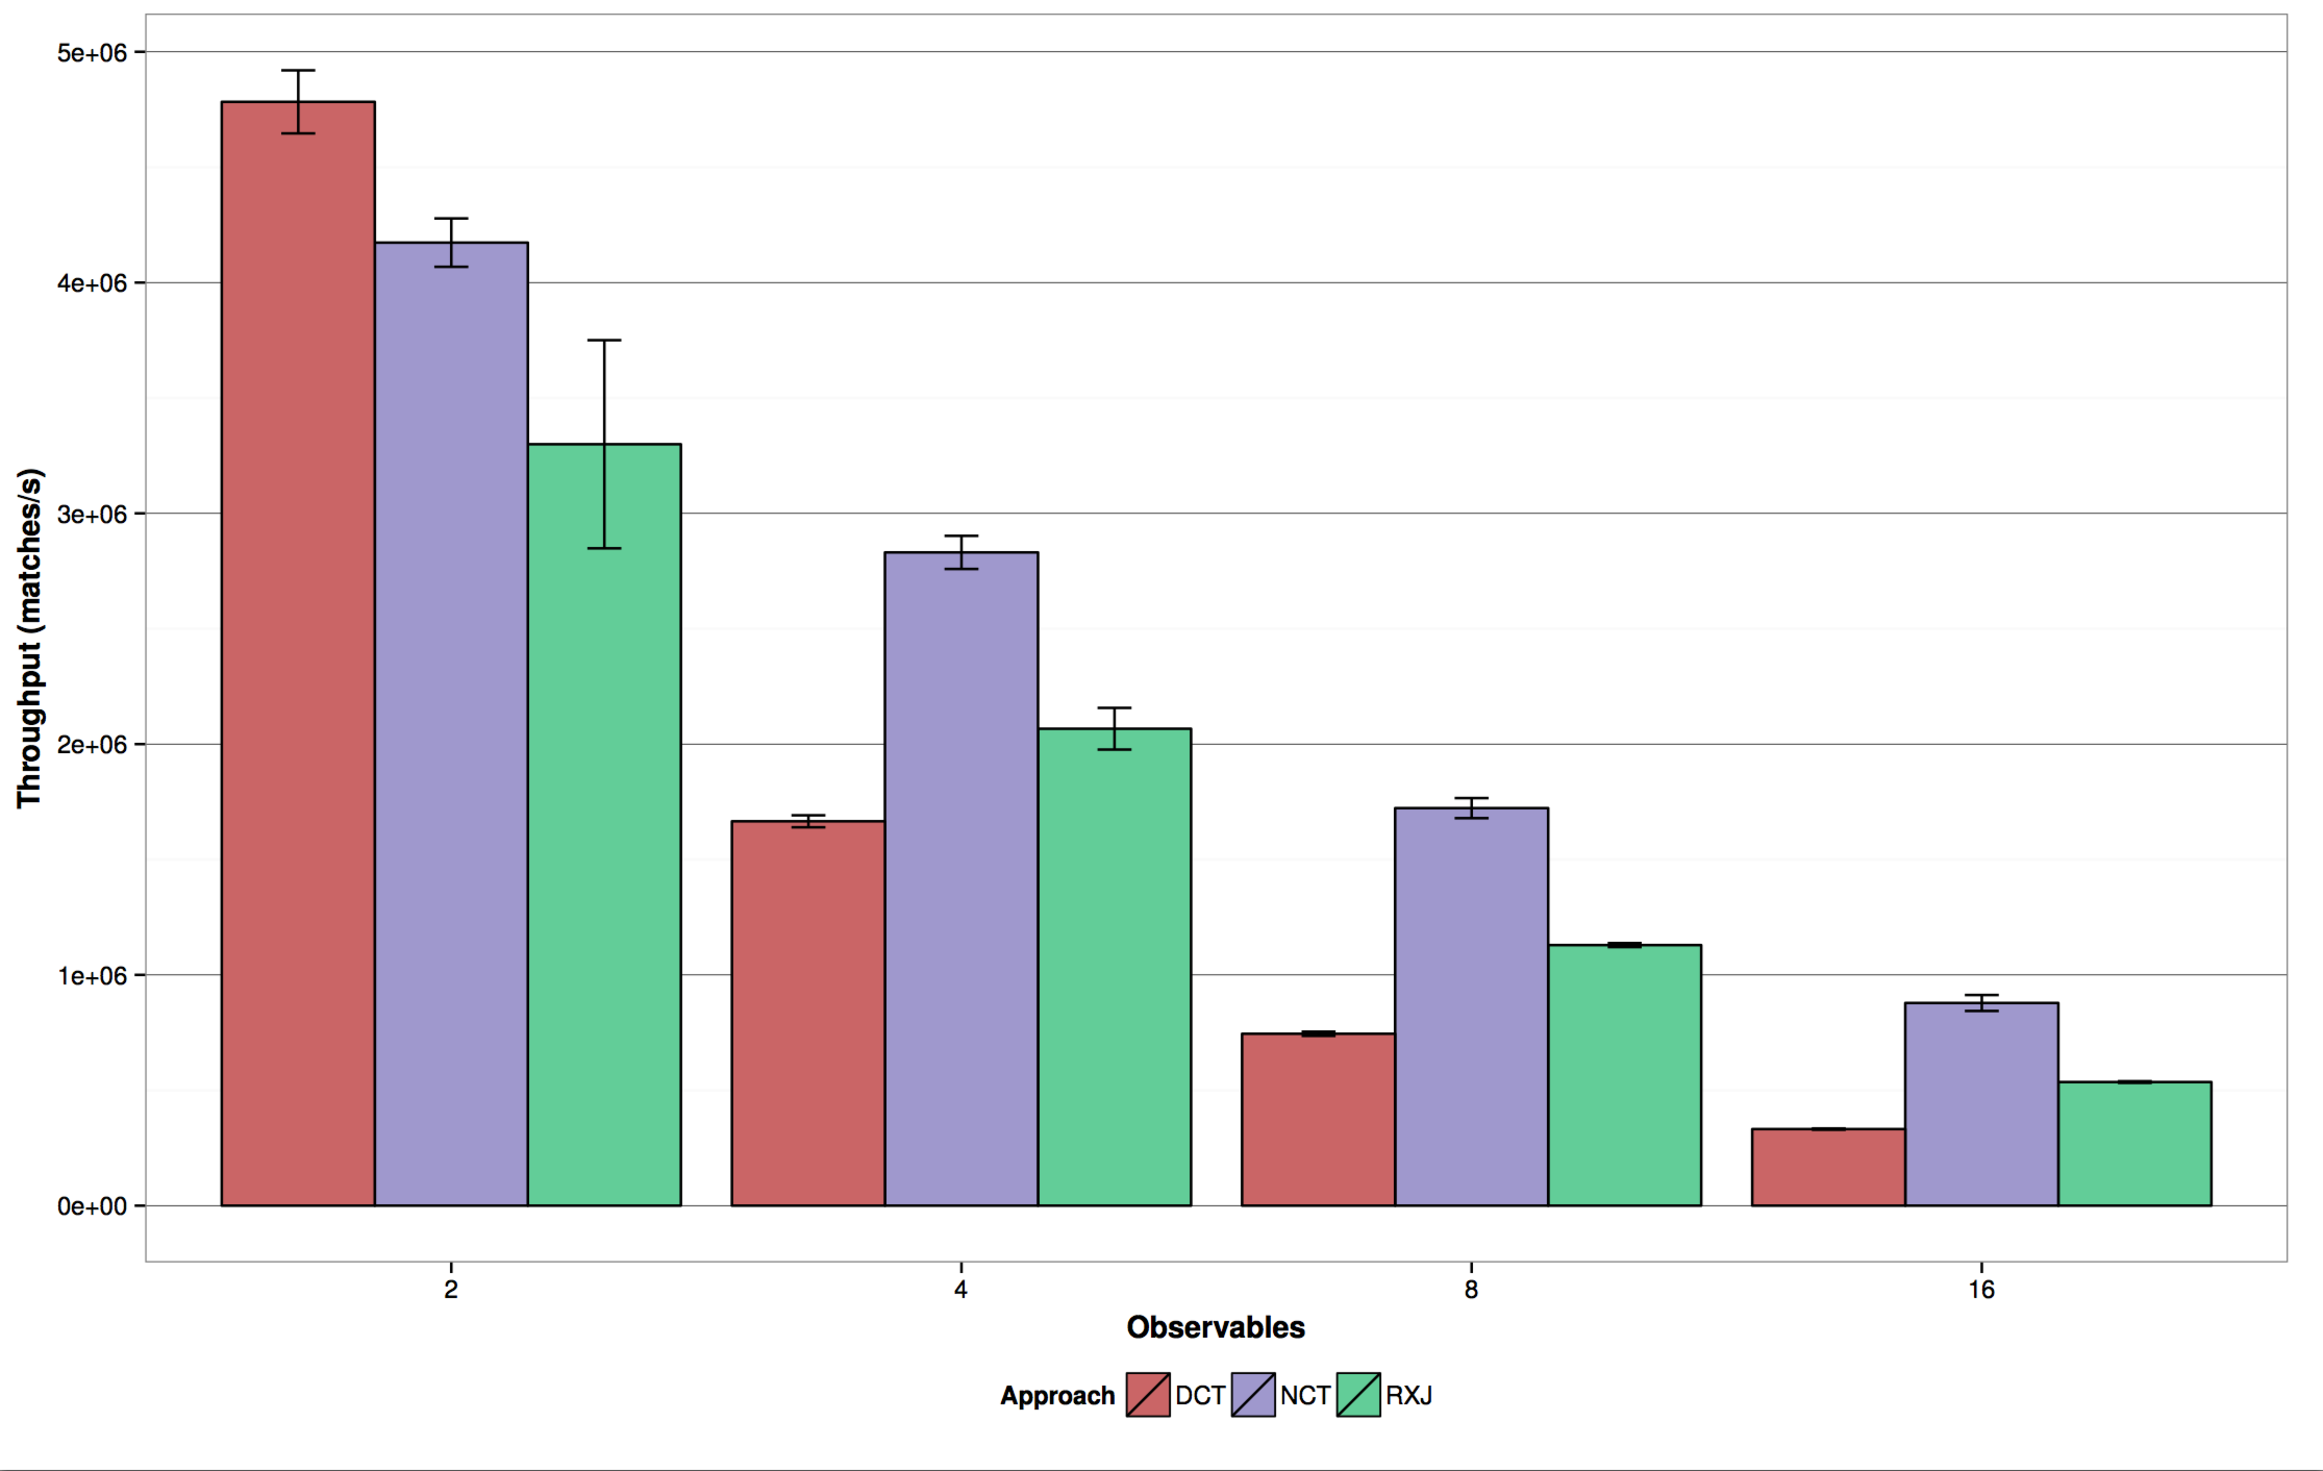
\includegraphics[scale=0.30]{img/two-patterns-N-observables.pdf}
  \caption{Matching two patterns with an increasing number of observables}
  \label{fig:TwoChoiceNObservables}
\end{figure}

As can be seen in Fig.~\ref{fig:TwoChoiceNObservables}, except for the case
of two cases with one observable each, the non-deterministic choice transform
(NCT) has highest throughput. Generally, throughput decreases roughly linearly
with increasing pattern sizes. The deterministic choice transform (DCT) has
lowest throughput with the exception of two observables shared between two
choices. The high throughput in this case is explained by the lazy-queuing
optimization applied by DCT. In this case no message is put into buffers by
DCT, whereas NCT and RXJ always put messages into buffers. The average
increase in throughput when using NCT over RXJ is 30.3\%.

\subsubsection{Throughput vs. number of patterns}

\begin{figure}[h]
  \centering
  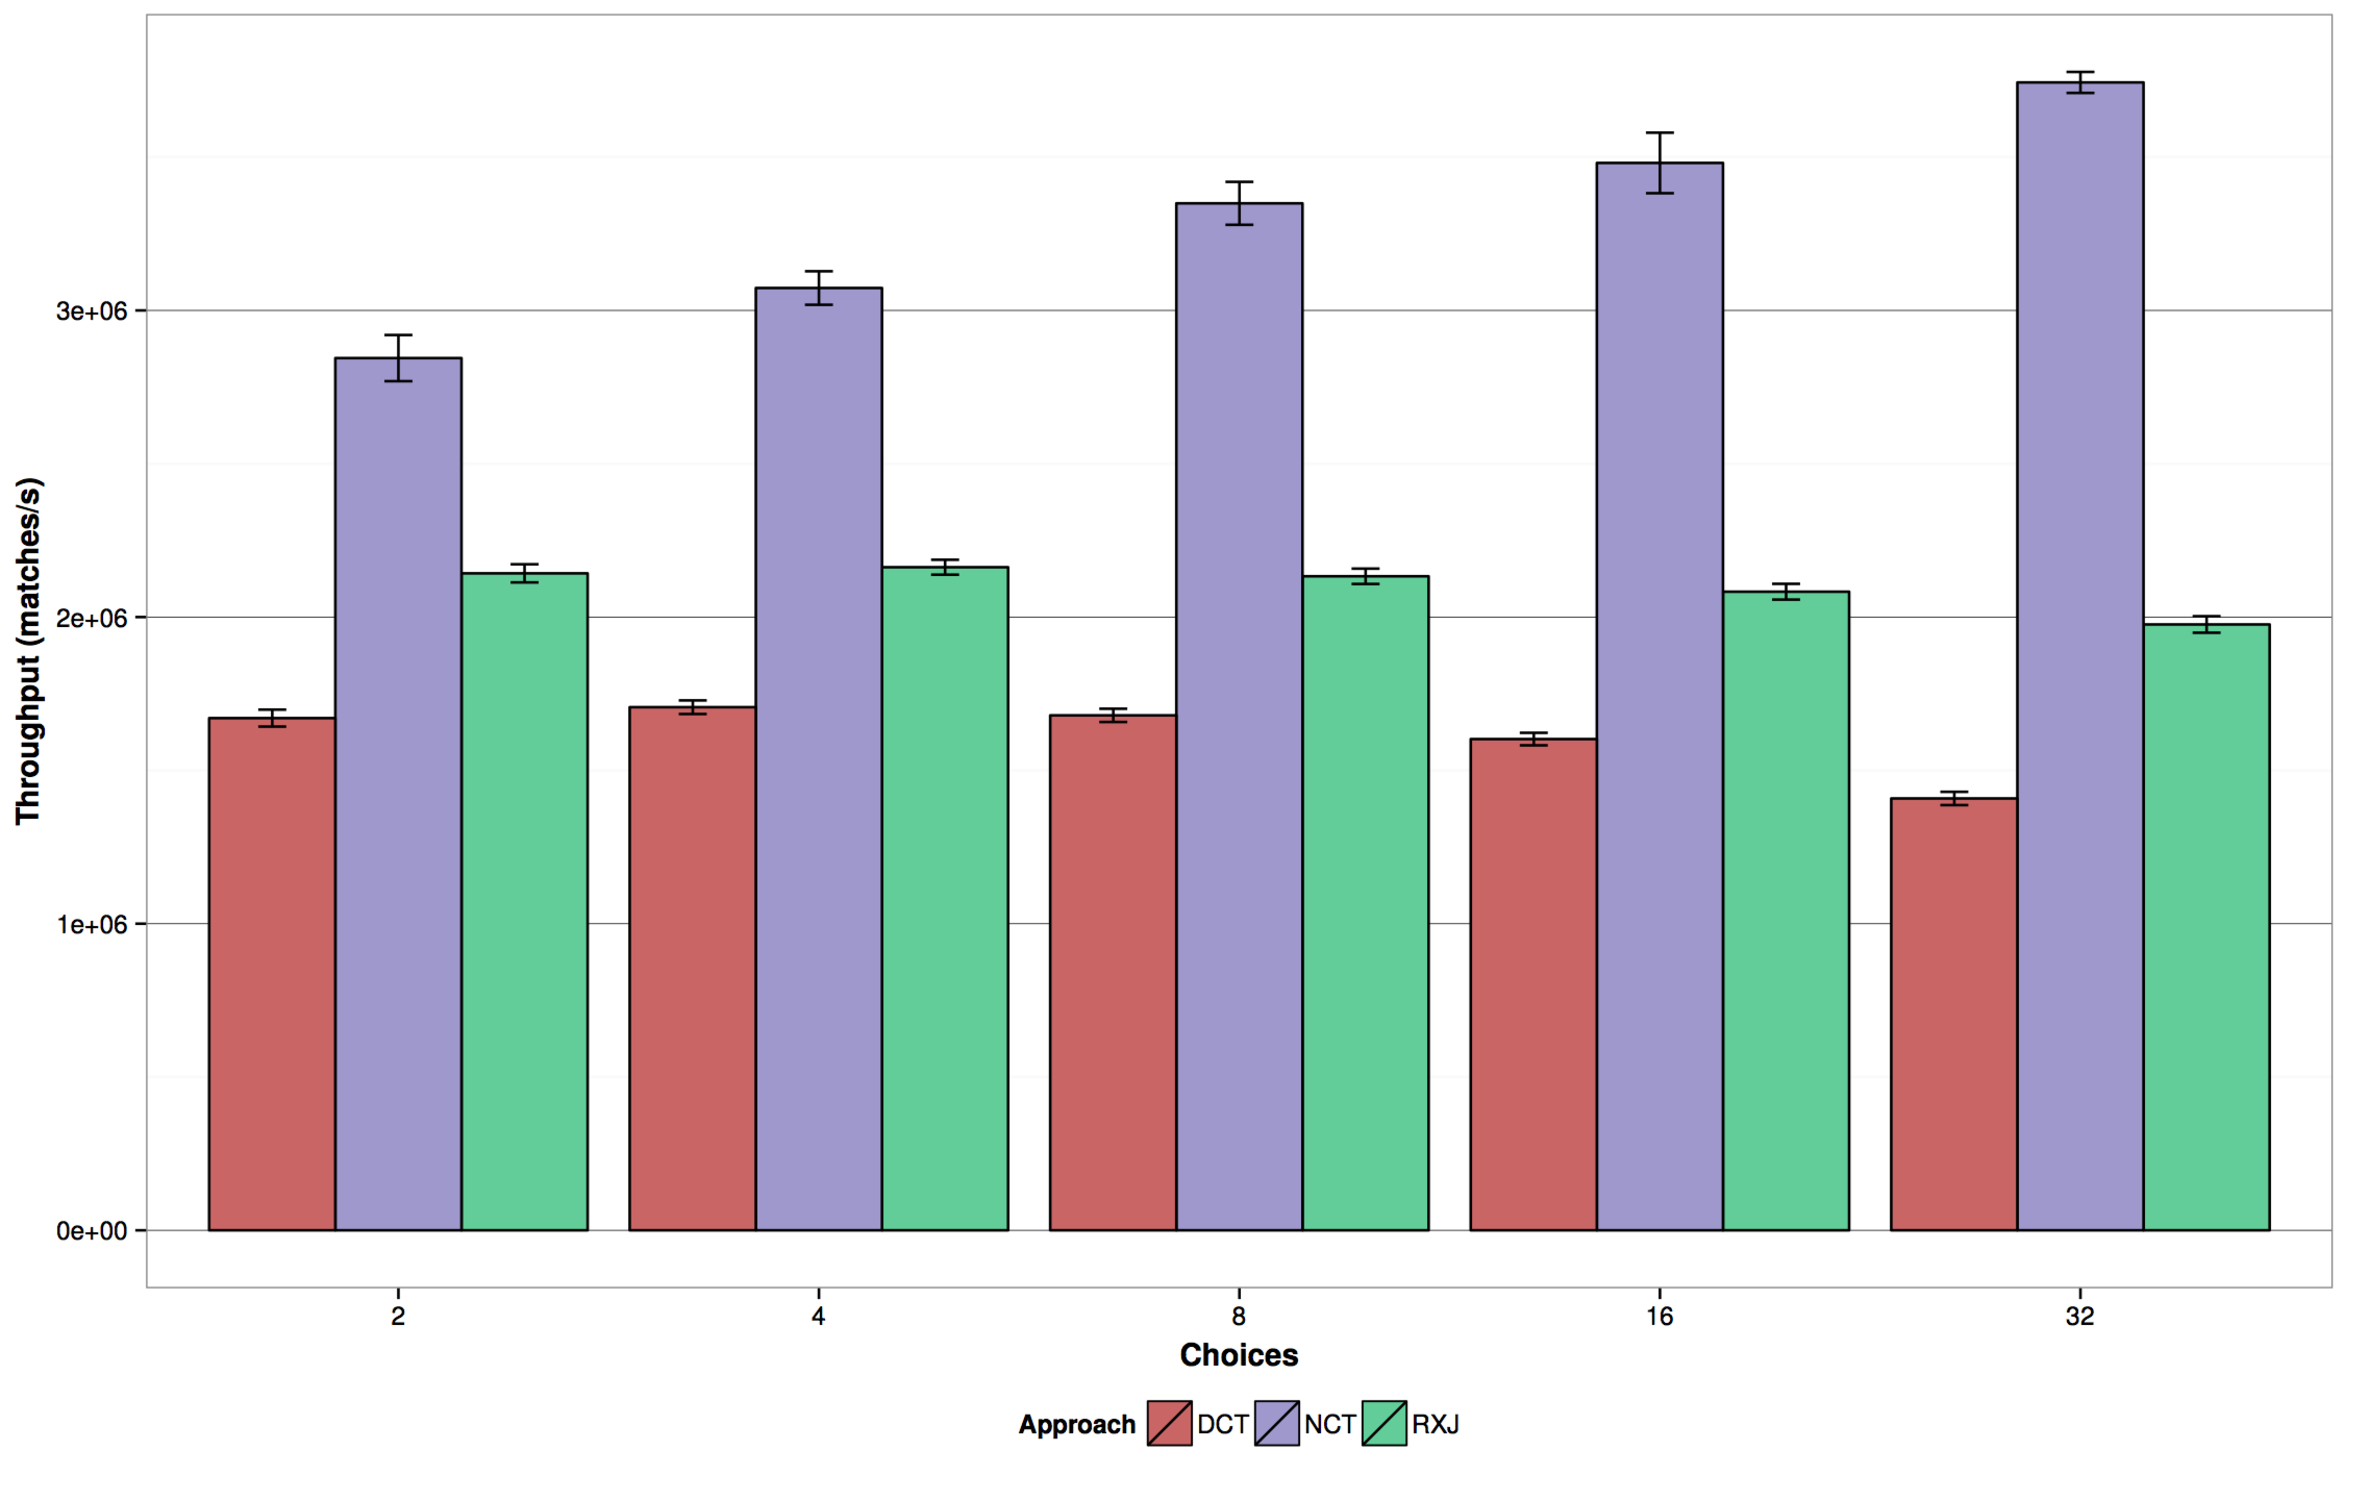
\includegraphics[scale=0.30]{img/N-patterns-two-observables.pdf}
  \caption{Matching an increasing number of patterns with two observables each}
  \label{fig:NChoiceTwoObservables}
\end{figure}

% \begin{figure}[t!]
% % \vspace{-4mm}
% \begin{subfigure}{.5\textwidth}
%   \centering
%   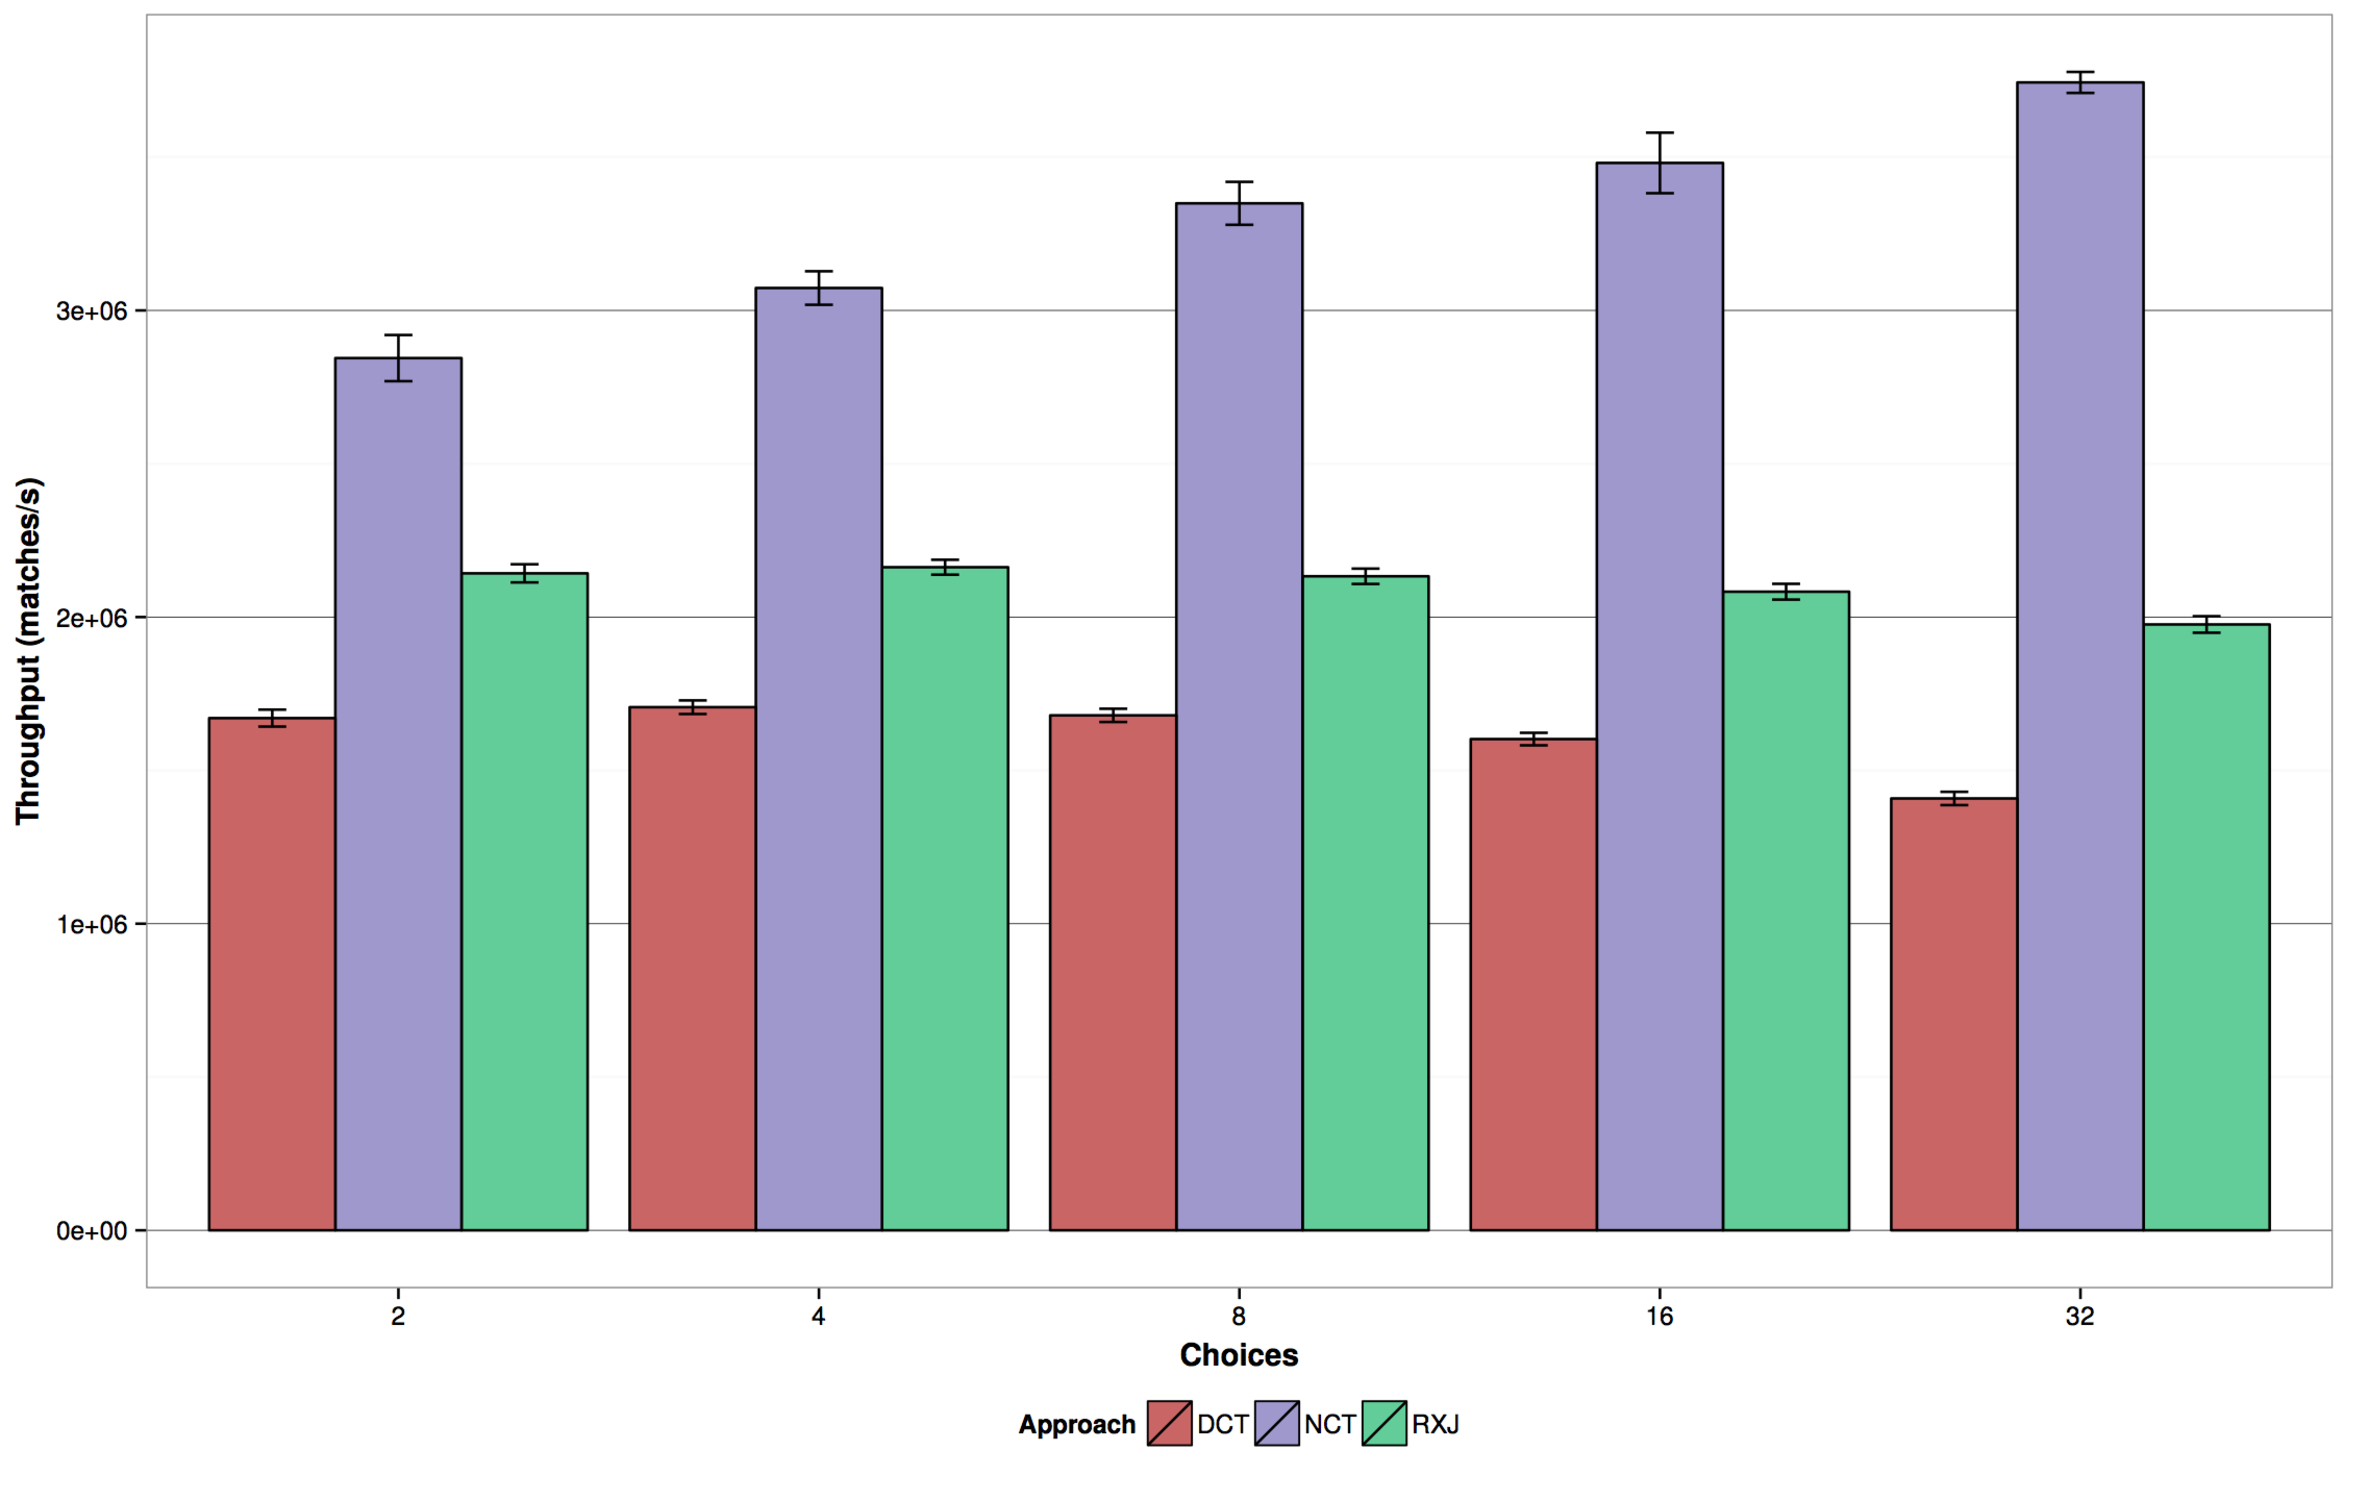
\includegraphics[scale=0.15]{img/N-patterns-two-observables.pdf}
%   \caption{Caption 1}
%   \label{fig:function-arity1}
% \end{subfigure}%
% \begin{subfigure}{.5\textwidth}
%   \centering
%   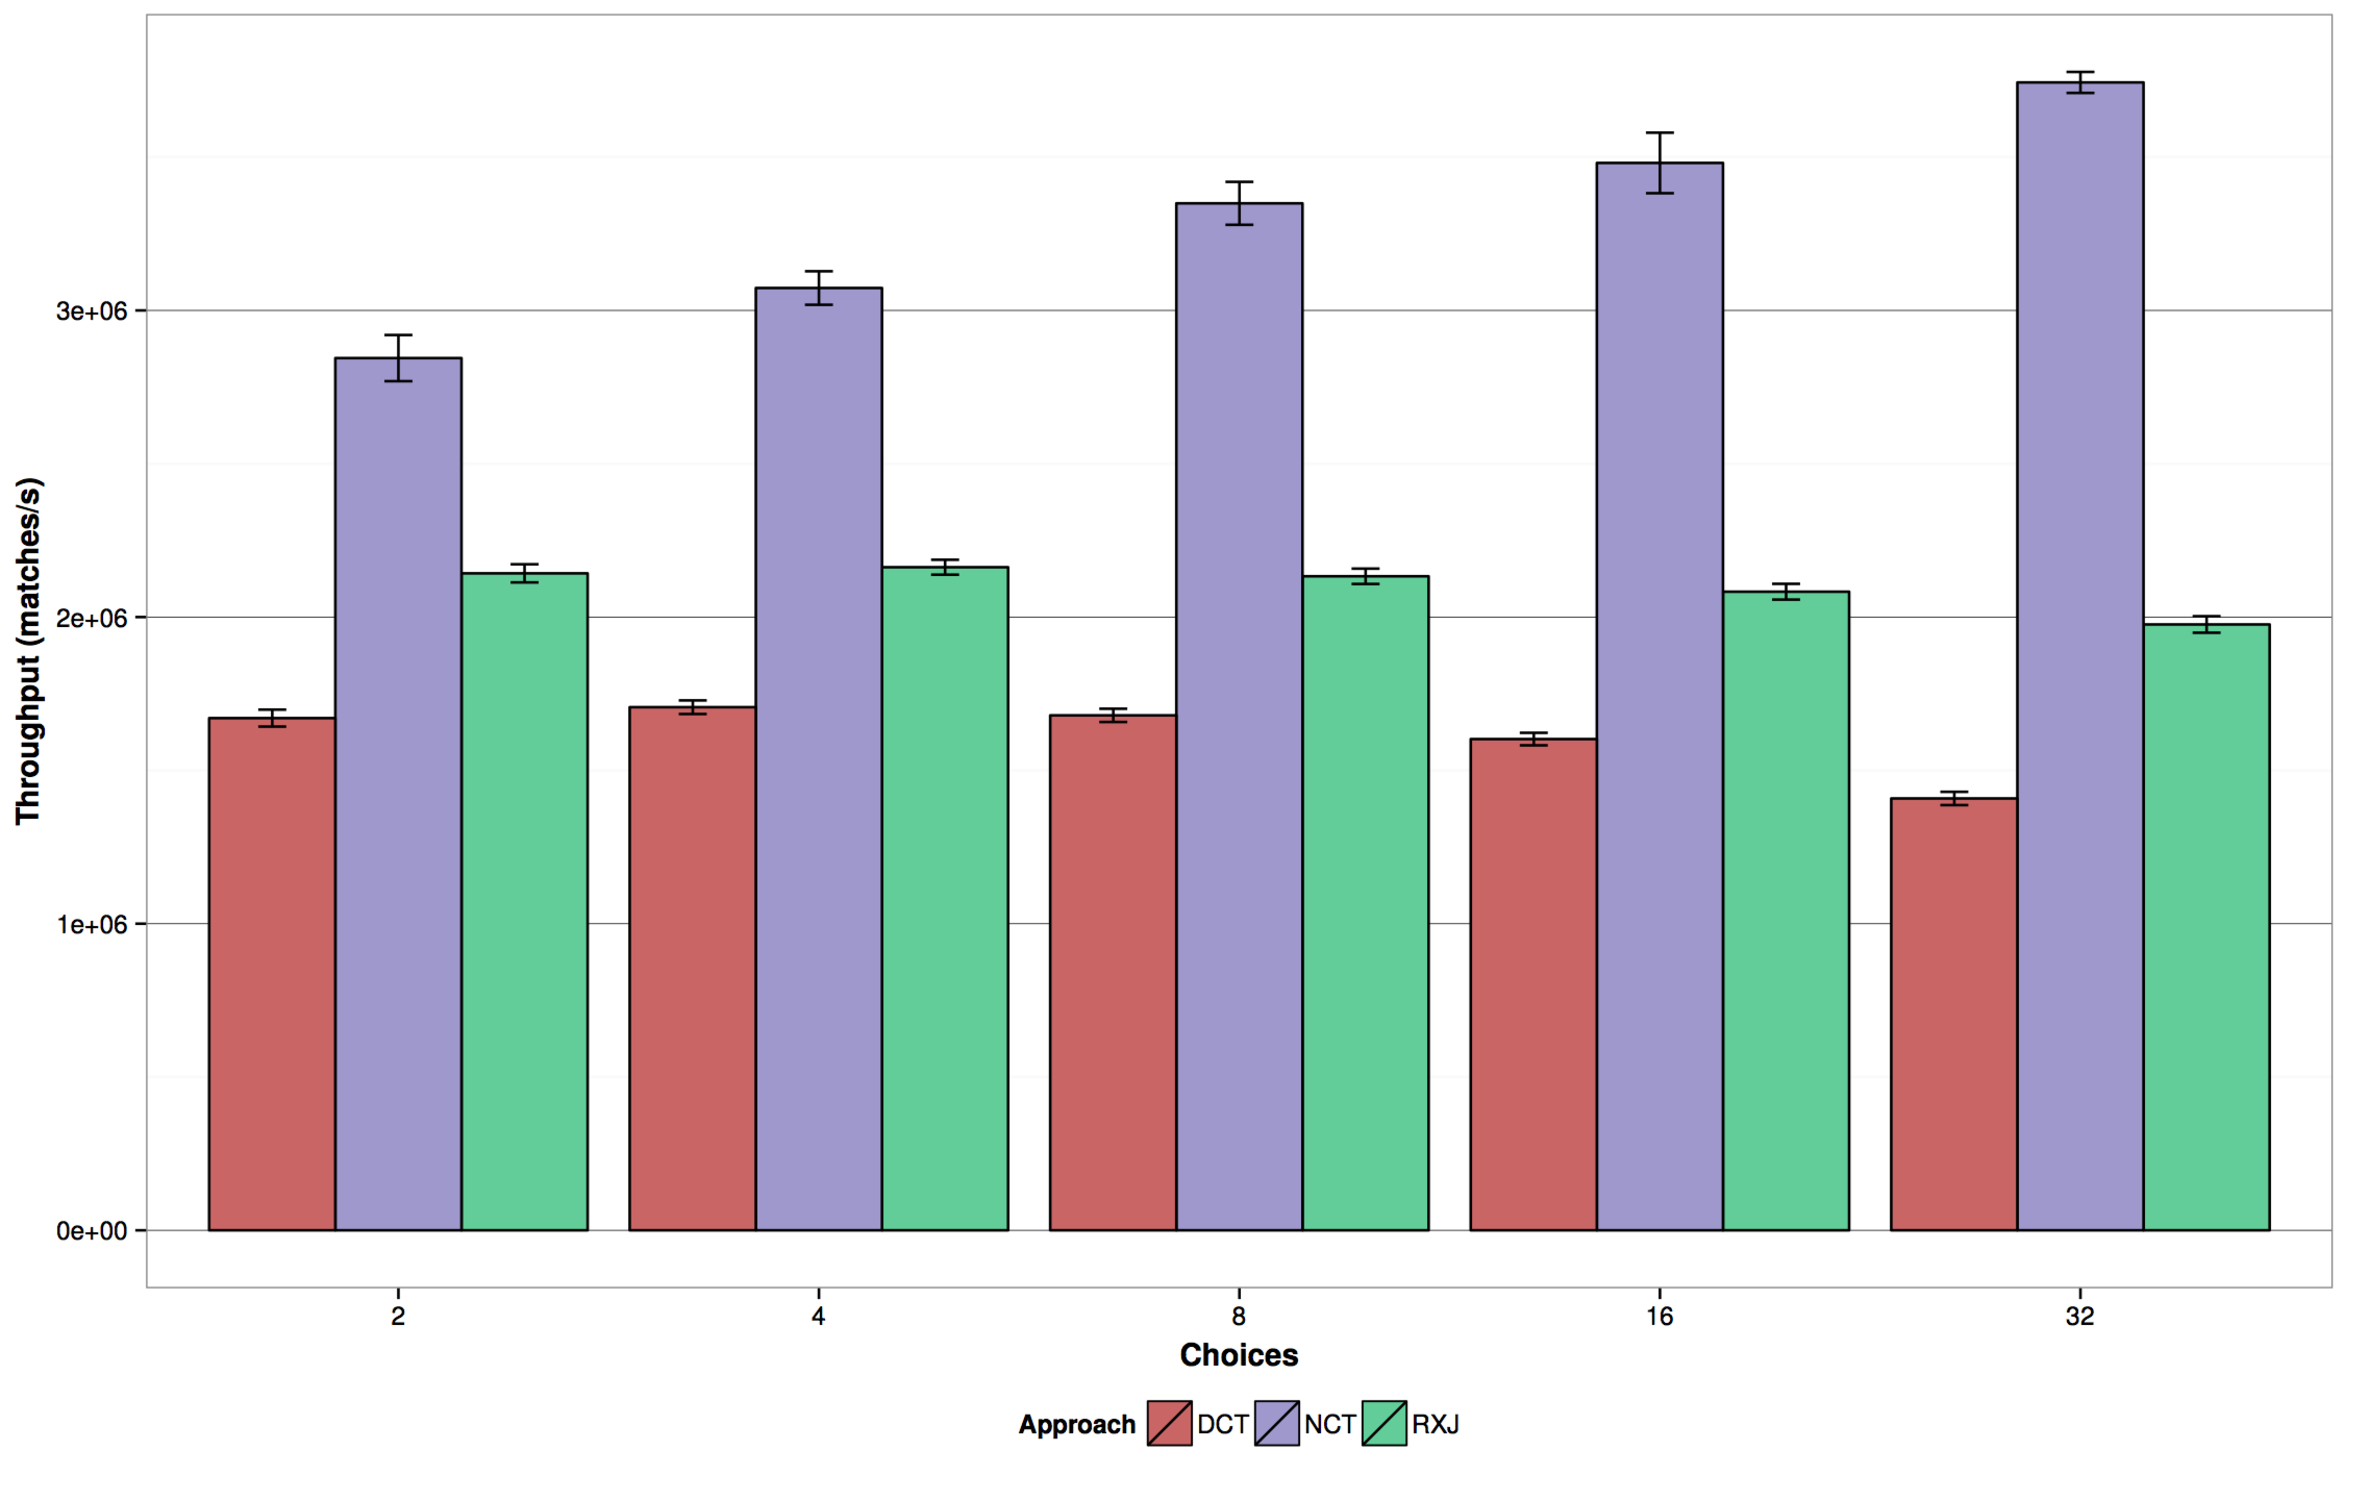
\includegraphics[scale=0.15]{img/N-patterns-two-observables.pdf}
%   \caption{Caption 2}
%   \label{fig:spore-arity1}
% \end{subfigure}%
% \vspace{1mm}
% \caption{Benchmark 2}
% \label{fig:bench2}
% \vspace{-2mm}
% \end{figure}



Performance with an increasing number of choices/patterns shows some
interesting results, as can be seen in Fig.~\ref{fig:NChoiceTwoObservables}.
The coarse-grained approaches DCT and RXJ have an almost constant throughput
with increasing number of choices whereas NCT achieves increased throughput.
This indicates that NCT leverages concurrency better than the other
approaches. The average increase in throughput of NCT over RXJ is 35.6\%.

\subsubsection{Performance with Increasing Size of Interdependentness}

\begin{figure}[h]
  \centering
  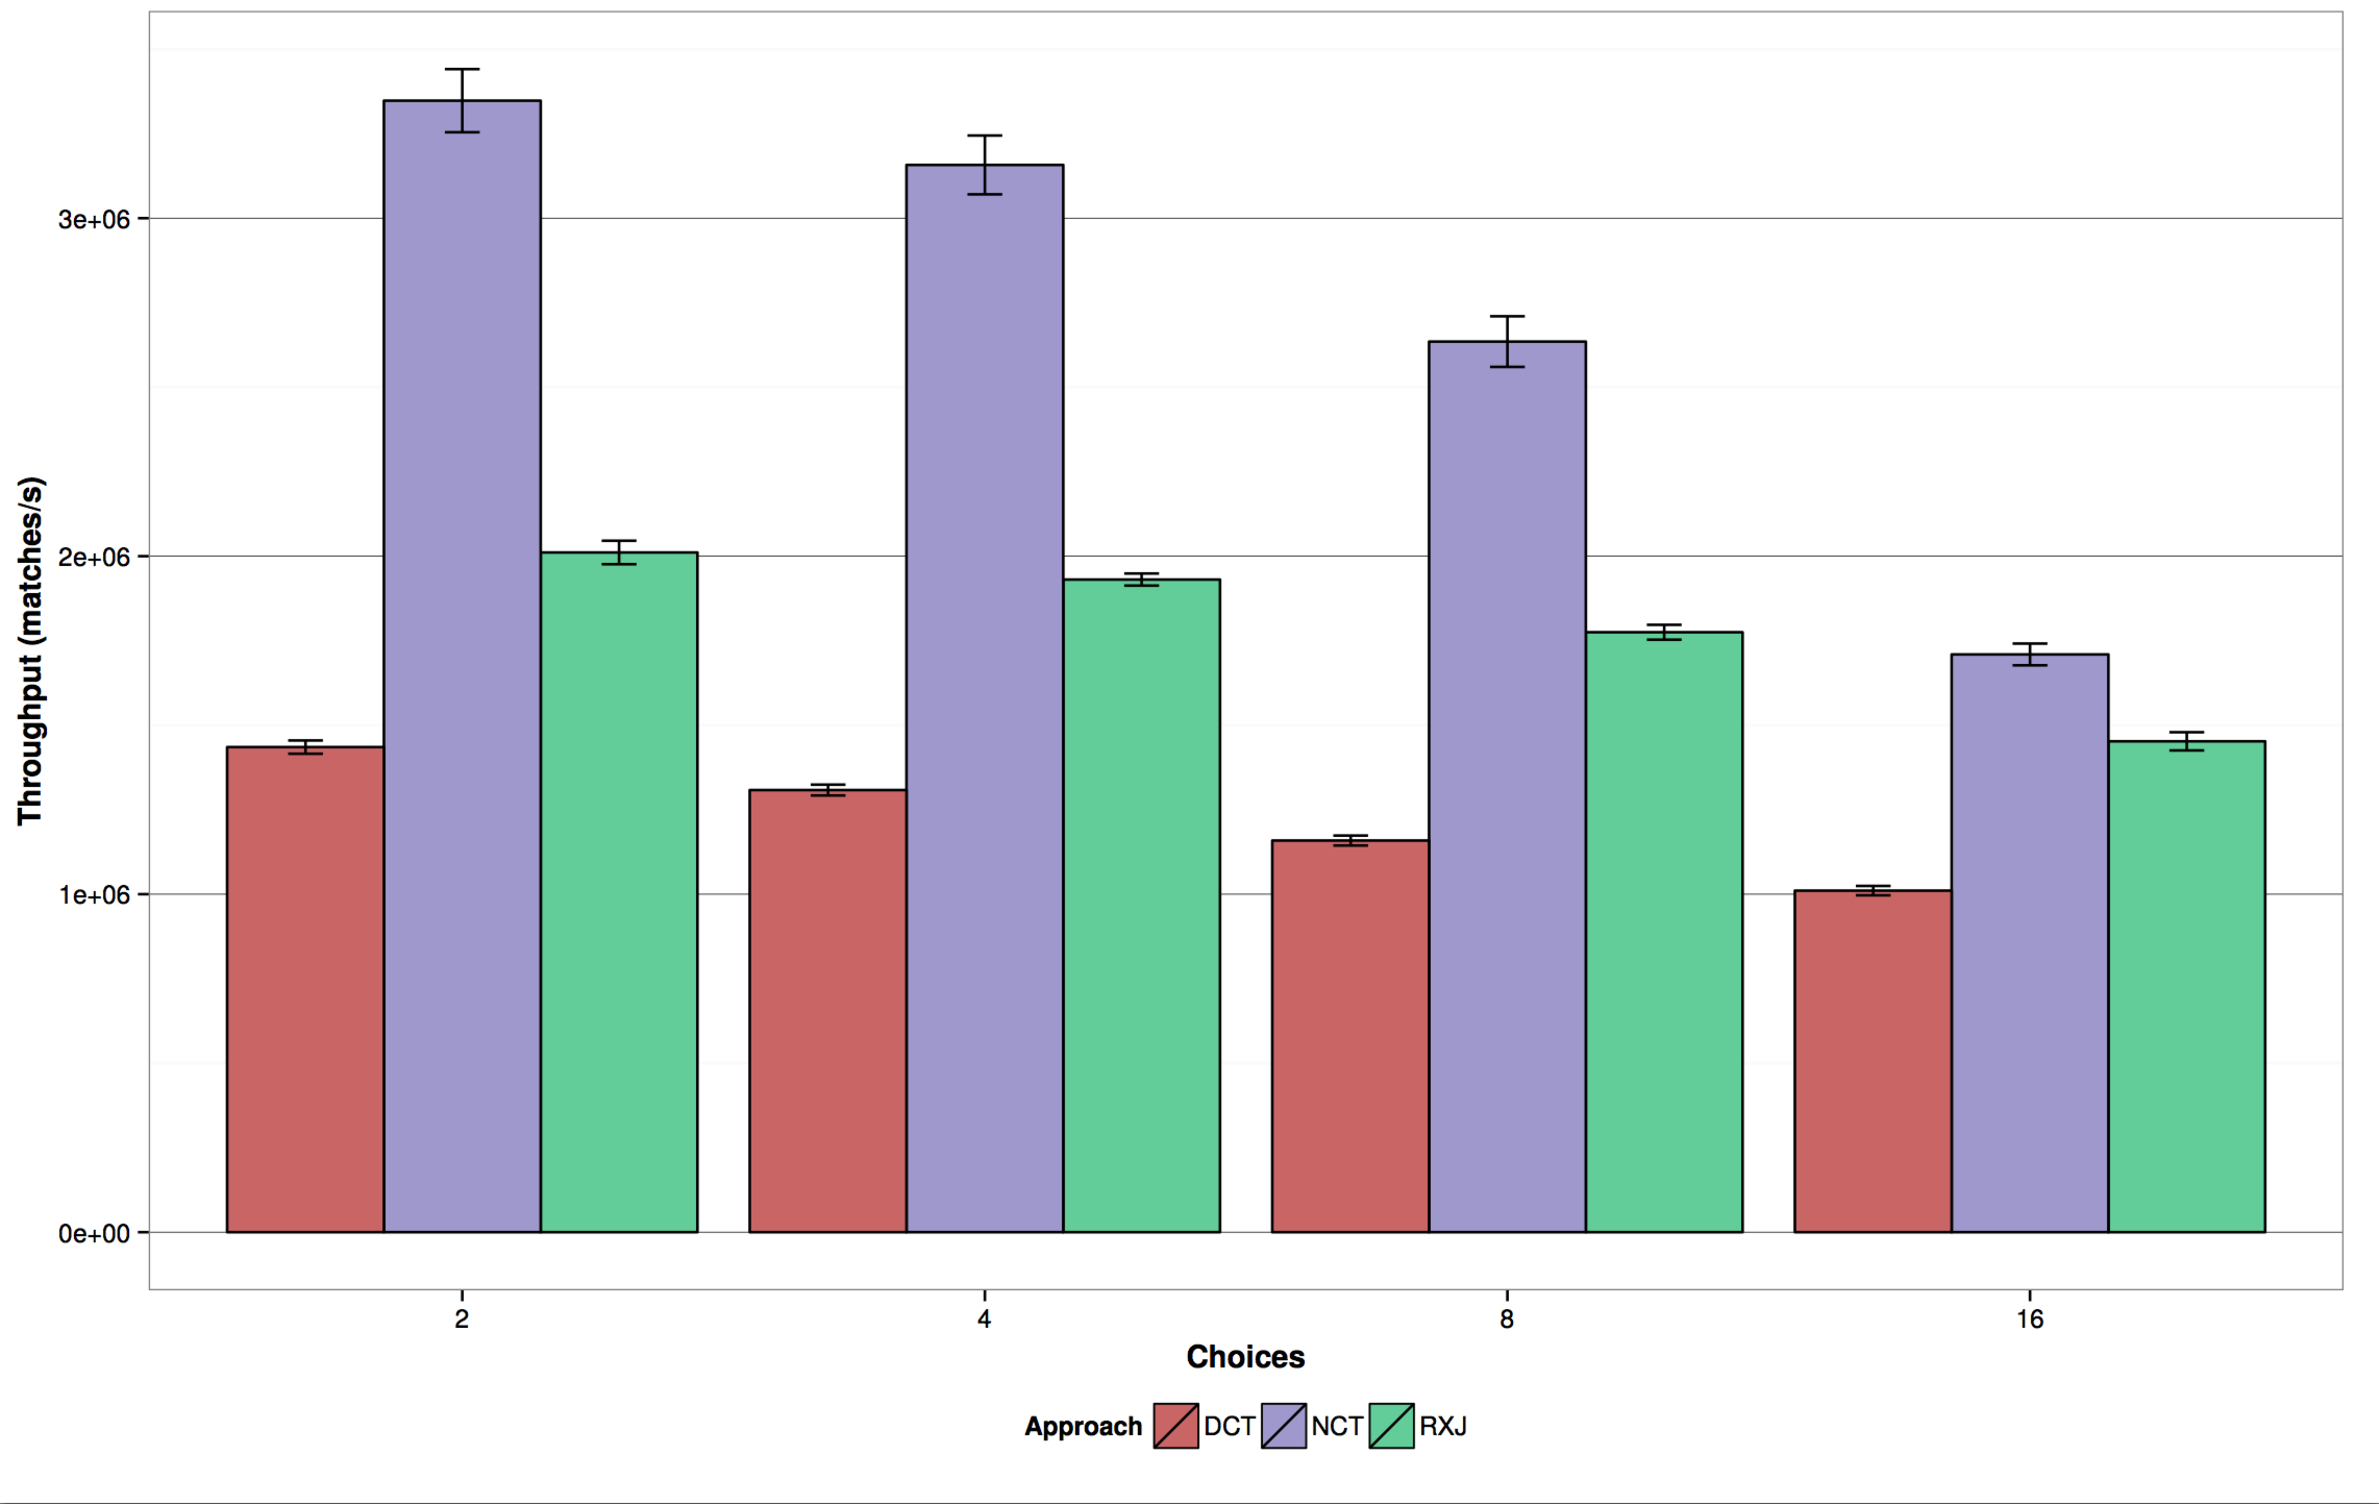
\includegraphics[scale=0.30]{img/32-patterns-N-interdep.pdf}
  \caption{}
  \label{fig:}
\end{figure}

The hypotheses that NCT leverages concurrency is supported by the
interdependentness tests: the throughput, while generally higher than the
other two approaches, does decrease with increasing number of interdependent
choices. The other two approaches remain more or less constant. The average
increase in throughput when using NCT over RXJ is 31.6\%.



\section{Conclusion}\label{sec:conclusion}

High-level synchronization constructs are indispensible for simplifying
asynchronous programming. In this paper we have proposed a scalable
synchronization construct based on the join-calculus. Our goal is an
integration with existing, stream-based programming models. For this purpose,
we have adapted Turon and Russo's scalable join-pattern matching algorithm to
work with the ordering constraints of streams. Micro benchmarks confirm the
benefits of fine-grained concurrency: on average, throughput of matching join
patterns increases by 30-36\% compared to the standard joins implementation of
\textsc{RxJava}, a state-of-the-art streaming implementation for the JVM.


\bibliographystyle{abbrv}
\bibliography{bib}

\end{sloppypar}
\end{document}
